\documentclass{standalone} 
\usepackage{tikz}
\usetikzlibrary{arrows,positioning,automata,shadows,fit,shapes}
\begin{document}
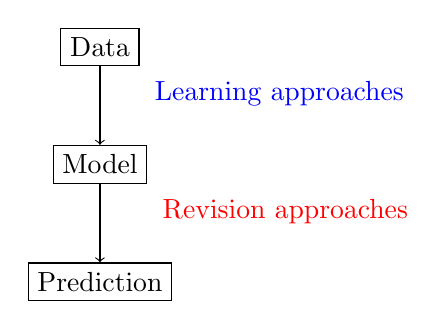
\begin{tikzpicture}
                    \node [draw](data) {Data};
                    \node [draw,below = of data] (model) {Model};
                    \draw[->] (data) -- (model);
                    \node [draw,below = of model] (pred) {Prediction};
                    \draw[->] (model) -- (pred);
                    \node [below right = 0.1cm of data] (LFIT){\textcolor{blue}{Learning approaches}};
                    \node [below right = 0.1cm of model] (Revision){\textcolor{red}{Revision approaches}};
\end{tikzpicture}
\end{document}
